\documentclass{article}

\usepackage[eandd]{neurips_2026}

\usepackage[utf8]{inputenc}
\usepackage[T1]{fontenc}
\usepackage{hyperref}
\usepackage{url}
\usepackage{booktabs}
\usepackage{amsfonts}
\usepackage{amsmath}
\usepackage{nicefrac}
\usepackage{microtype}
\usepackage{xcolor}
\usepackage{graphicx}
\usepackage{multirow}

\title{Comparing Inference-Time Methods for Natural-Language Mathematical Proofs}

\author{%
  Anonymous Author(s)
}

\begin{document}

\maketitle

\begin{abstract}
We compare inference-time scaffolding methods for mathematical proof generation against
plain sampling at matched cost.
On 70 problems (60 IMO-ProofBench + 10 frontier-tier 2026 research items),
six base models, four architectures, and three automated judges under a
{\raise.17ex\hbox{$\scriptstyle\sim$}}\$1{,}000 budget:
(1)~the generator-verifier-revisor pipeline does not beat pass@3 under either strict
judge ($\Delta{=}{-}0.08$, problem-clustered 95\% CI $[{-}0.25, {+}0.08]$, $p{=}0.36$);
(2)~seeded-ideator-plus-pipeline shows a positive effect concentrated at reasoning=max
on cheap models (cluster $\Delta{=}{+}0.60$, $p{=}0.005$; partial coverage, no cell
survives Holm correction);
(3)~judge choice flips conclusions: the lenient judge calls ``pass'' on 37\% of
strict-fail cases;
(4)~pass-rate degrades from 86\% at pre-competition to 0\% at research-frontier;
(5)~pooling 3{,}178 trials yields 32 strict-judge candidate passes on 2026 research
problems, 23 on a single likely-contaminated item.
The recommendation: draw more samples before adding pipeline depth, keep reasoning on,
and audit with judges of different leniency.
\end{abstract}

%% ============================================================
\section{Introduction}
\label{sec:intro}

Language models have moved from saturating school-math benchmarks to plausibly
contributing to research mathematics.
AlphaProof achieved IMO silver in 2024~\citep{hubert2025alphaproof};
gold-tier systems from DeepMind~\citep{deepmind2025deepthink},
OpenAI~\citep{wei2025openaiimo}, and Harmonic~\citep{achim2025aristotle} followed
in 2025; and the Erd\H{o}s repository now lists dozens of model-assisted
contributions~\citep{tao2026erdos,erdosproblems}.

Two methodological gaps motivate this work.
First, comparing a multi-call pipeline against pass@1 is unfair: the proper
baseline is pass@$n$ matched to the pipeline's call budget, not pass@1.
We use measured per-trial cost to set this matching (\S\ref{sec:arch}).
Second, evaluation of free-form proofs at scale relies on automated judges, and
the gap between lenient and strict judges is large enough to flip qualitative
conclusions about which architecture wins.

A third constraint shaped every choice: a {\raise.17ex\hbox{$\scriptstyle\sim$}}\$1{,}000
OpenRouter budget, which kept us off frontier-tier generators and judges and forced
partial coverage of the most expensive architecture.

We do not propose a new method.
We characterize a six-by-four-by-three space (model $\times$ architecture $\times$
judge) on a 70-problem benchmark and audit what holds up under paired bootstrap CIs
and permutation tests.
Contributions:
\begin{enumerate}
\setlength\itemsep{0pt}
\item A token-cost-fair, statistically tested comparison of pass@$k$ against
  generator-verifier-revisor pipelines and seeded-ideator variants, stratified by
  difficulty.
\item Quantification of judge-induced variance: cell-level CIs on the
  strict-vs-lenient false-positive rate.
\item A frontier-solves audit pooling 3{,}178 trials with per-problem breakdowns.
\item Reproducible per-experiment artifacts totaling {\raise.17ex\hbox{$\scriptstyle\sim$}}3{,}200 trial rows.
\end{enumerate}

%% ============================================================
\section{Related work}
\label{sec:related}

\paragraph{Capability arc.}
The trajectory from GSM8K and MATH~\citep{hendrycks2021math} through IMO
competitions includes AlphaProof~\citep{hubert2025alphaproof}, Deep
Think~\citep{deepmind2025deepthink}, Aristotle~\citep{achim2025aristotle}, and an
open-source agentic framework~\citep{huang2025imogold}.
Through early 2026, models produced solutions on the Erd\H{o}s
repository~\citep{tao2026erdos,feng2026erdos}, on FrontierMath open
problems~\citep{glazer2024frontiermath}, and via Aletheia~\citep{feng2026aletheia}.

\paragraph{Benchmarks.}
IMO-ProofBench~\citep{luong2025imobench}: 30 Basic + 30 Advanced olympiad proofs
with a hardened grader ($r{=}0.96$ to human judges).
We augment with ten 2026 research problems (Erd\H{o}s 333, 397, 654, 659, 1051;
FirstProof 4, 5, 6, 10~\citep{abouzaid2026firstproof}; Epoch's Ramsey-hypergraph
problem) and call the union PB+R26.

\paragraph{Architectures.}
Pass@$k$~\citep{brown2020gpt3,chen2021codex}: sample $k$ solutions, take best.
Self-consistency~\citep{wang2022selfconsistency} and chain-of-thought~\citep{wei2022cot}
are established baselines.
Generator-verifier-revisor pipelines appear in
Aletheia~\citep{feng2026aletheia} and Huang--Yang~\citep{huang2025imogold}.
We restrict to natural-language proofs; we do not study formal
verification, evolutionary search~\citep{novikov2025alphaevolve,georgiev2025exploration},
or hybrid neuro-symbolic systems.

%% ============================================================
\section{Methodology}
\label{sec:method}

\subsection{Architectures}
\label{sec:arch}

We implement four architectures in a single pipeline with shared model-call
infrastructure, using prompts derived from Aletheia~\citep{feng2026aletheia} and
Huang--Yang~\citep{huang2025imogold}.
Final grading uses the IMO-ProofBench judge prompt, restricted to $\{0,1,6,7\}$.

\begin{itemize}
\setlength\itemsep{1pt}
\item \textbf{Pass@$k$.} Run $k$ independent generations; take max judge score.
  We sweep $k \in \{1,3\}$ in the main comparison, $k \in \{1,3,5,7,9\}$ in the
  scaling experiment. The \texttt{generate} mode produces 3 branches per trial
  (i.e., pass@3).
\item \textbf{Generator-verifier-revisor (\texttt{full}).} Up to three
  verifier-revisor iterations; early-stop on \texttt{VERDICT:~correct}.
\item \textbf{Seeded ideator (\texttt{seed\_generate}).} An ideation call produces
  three sketch directions; each is realized as a full solution.
\item \textbf{Ideator + pipeline (\texttt{seed\_full}).} Each ideated seed runs
  through the verifier-revisor loop.
\end{itemize}

\paragraph{Empirical cost matching.}
Median measured per-trial cost gives \texttt{full} at $0.78\times$
\texttt{generate}, \texttt{seed\_generate} at $1.00\times$, and \texttt{seed\_full}
at $1.36\times$---far short of the nominal $3\times$ and $9\times$ (verifier/revisor
calls are shorter and \texttt{full} early-stops on easy problems).
Cost-matching: \texttt{full} and \texttt{seed\_generate} $\approx$ pass@3;
\texttt{seed\_full} $\approx$ pass@4--5, not pass@9.

\subsection{Models, reasoning, and dataset}

Six cost-feasible base models: DeepSeek-v4-flash, -pro, Gemini-3-flash-preview,
Gemma-4-31B-IT, GPT-OSS-120B, Qwen3.6-35B-A3B.
Gemma-4 and GPT-OSS additionally run with reasoning=max.
Table~\ref{tab:tiers} shows the difficulty stratification.

\begin{table}[t]
  \caption{Problem set and difficulty tiers. PB = ProofBench; R26 = 2026 research problems.}
  \label{tab:tiers}
  \centering
  \small
  \begin{tabular}{llr}
    \toprule
    Tier & Source & $n$ \\
    \midrule
    pre-competition ($d{=}0$) & PB-Basic & 30 \\
    competition-hard ($d{=}1$) & PB-Advanced + Erd\H{o}s~397 & 31 \\
    research-easy ($d{=}2$) & Erd\H{o}s~333, 654, 659; FirstProof~10 & 4 \\
    research-medium ($d{=}3$) & Erd\H{o}s~1051; FirstProof~5 & 2 \\
    research-hard ($d{=}4$) & FirstProof~4, 6 & 2 \\
    research-frontier ($d{=}5$) & Ramsey hypergraphs & 1 \\
    \bottomrule
  \end{tabular}
\end{table}

\subsection{Judges}

Three judges score every architecture trial: DeepSeek-v4-flash (canonical),
DeepSeek-v4-pro (strict audit), and Gemini-3-flash-preview (lenient audit).
Section~\ref{sec:calibration} reports the GradingBench calibration.

\subsection{Statistical methodology}

Paired comparisons use within-(model, reasoning, problem) score differences.
\emph{Problem-clustered} CIs (used for headlines) resample whole problems with
replacement; 5{,}000 resamples, seed 20260507.
$p$-values are sign-flip permutation tests (10{,}000 permutations); the cluster
variant flips at the problem level.
For \S\ref{sec:seedfull}'s eight-test family we report Holm-corrected $p$-values.
Pass-rate CIs use Wilson; zero-pass cells use the one-sided 95\%
Clopper--Pearson upper bound.

%% ============================================================
\section{Calibration}
\label{sec:calibration}

\paragraph{Judge calibration on GradingBench.}
We tested ten judge configurations on 200 GradingBench problems (prompt restricted
to $\{0,1,6,7\}$).
DeepSeek-v4-flash achieves 87.4\% pass-agreement at \$0.004/call, on the Pareto
frontier of accuracy vs.\ cost (Figure~\ref{fig:pareto}).
The next-best judges cost 3.8--9.5$\times$ more;
Gemini-3-flash-preview agrees only 64\% at \$0.016/call.
Full results are in Appendix~\ref{app:gradingbench}.

\begin{figure}[t]
  \centering
  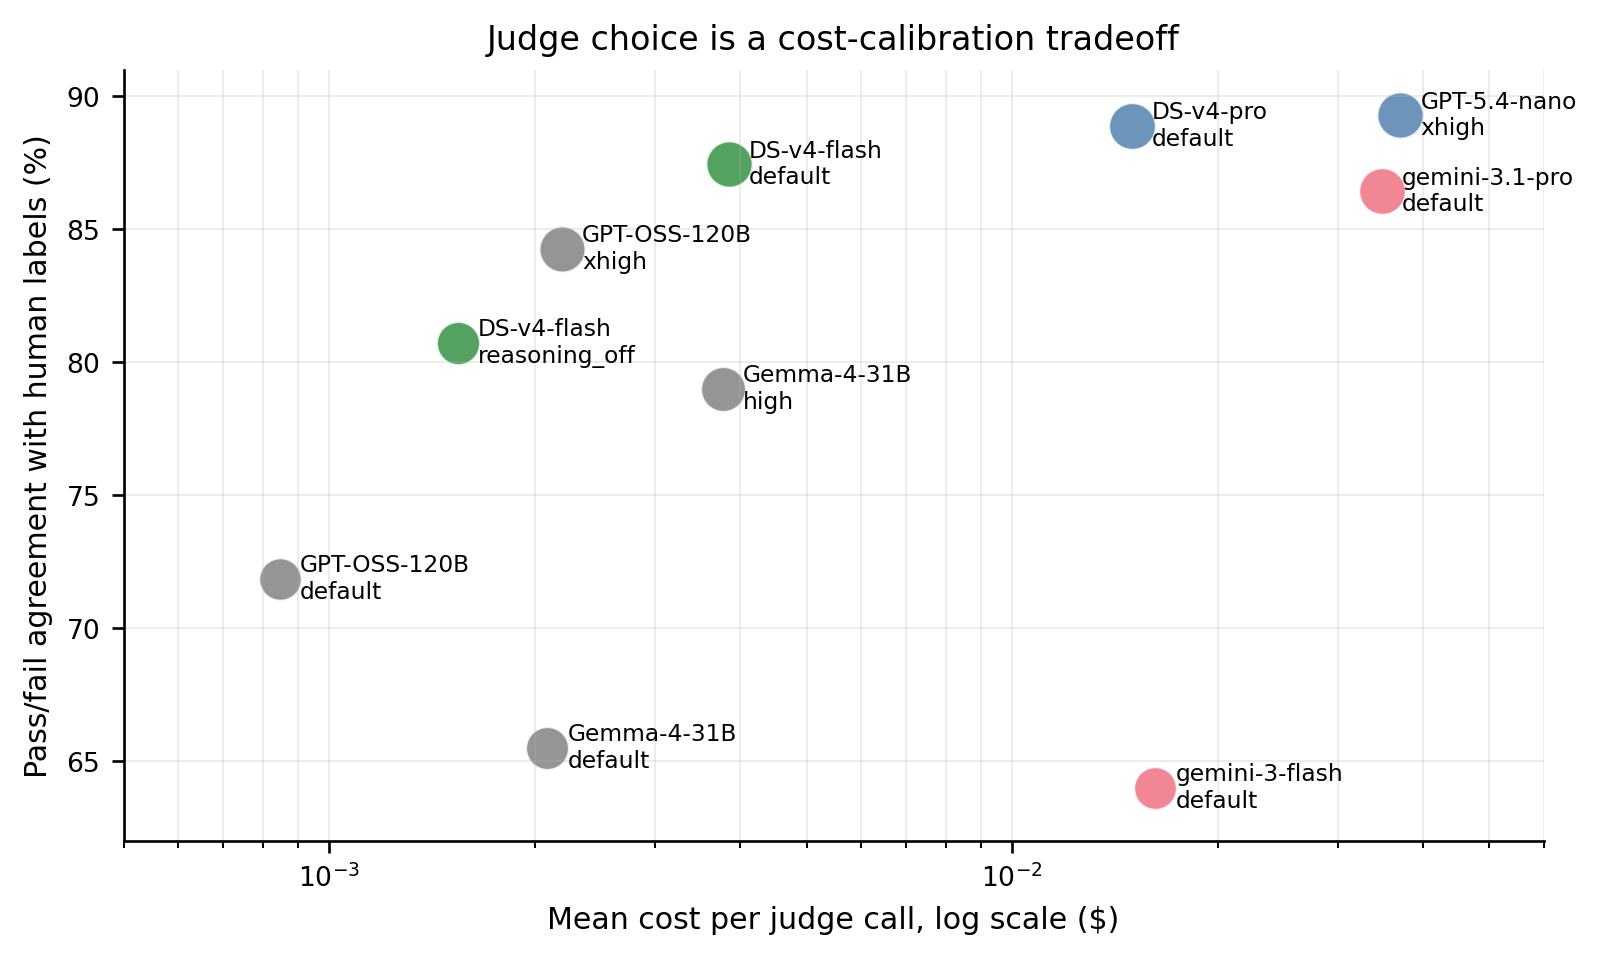
\includegraphics[width=0.65\textwidth]{plots/fig2_judge_calibration_pareto.png}
  \caption{Judge cost--calibration Pareto front on GradingBench ($n{=}200$).
    DeepSeek-v4-flash (green, top-left cluster) is the only high-agreement judge
    below \$0.01/call.}
  \label{fig:pareto}
\end{figure}

\paragraph{Generator selection on AnswerBench.}
Thirteen model--reasoning configurations on AnswerBench-50 (50 verifiable-answer
problems).
Reasoning is the dominant variable: GPT-OSS-120B jumps from 58\% to 74\%,
Gemini-3-flash from 74\% to 90\%.
Six models cleared 60\% accuracy; all six enter the architecture sweep
(Appendix~\ref{app:answerbench}).

%% ============================================================
\section{Main results}
\label{sec:results}

\subsection{Architecture comparison}
\label{sec:archcomp}

Table~\ref{tab:arch} shows pooled results across base models on PB+R26 under the
v4-flash judge.
Coverage is complete (6/6) for \texttt{generate}, \texttt{seed\_generate},
\texttt{full}; partial (3/6) for \texttt{seed\_full}.

\begin{table}[t]
  \caption{Architecture comparison (pooled, v4-flash judge). Top: aggregate
    statistics with Wilson pass-rate CIs. Bottom: paired contrasts with
    problem-clustered bootstrap.}
  \label{tab:arch}
  \centering
  \small
  \begin{tabular}{lccrrr}
    \toprule
    Mode & cost & coverage & $n$ & mean & pass rate \\
    \midrule
    pass@1 & $0.33\times$ & 6/6 & 613 & 1.97 & 0.28\,[0.25,\,0.32] \\
    \texttt{generate} (= pass@3) & $1.00\times$ & 6/6 & 543 & 2.31 & 0.33\,[0.29,\,0.37] \\
    \texttt{seed\_generate} & $1.00\times$ & 6/6 & 555 & 2.29 & 0.33\,[0.29,\,0.37] \\
    \texttt{full} & $0.78\times$ & 6/6 & 550 & 2.24 & 0.32\,[0.28,\,0.36] \\
    \texttt{seed\_full} \emph{(partial)} & $1.36\times$ & 3/6 & 344 & 2.58 & 0.37\,[0.32,\,0.42] \\
    \midrule
    \multicolumn{2}{l}{Contrast} & $n$ / problems & $\Delta$ & cluster 95\% CI & $p$ \\
    \midrule
    \multicolumn{2}{l}{\texttt{full} $-$ \texttt{generate}} & 533\,/\,70 & $-$0.08 & [$-$0.25,\,+0.08] & 0.36 \\
    \multicolumn{2}{l}{\texttt{seed\_gen} $-$ \texttt{generate}} & 539\,/\,70 & $-$0.03 & [$-$0.21,\,+0.16] & 0.78 \\
    \multicolumn{2}{l}{\texttt{seed\_full} $-$ \texttt{gen.} \emph{(partial)}} & 337\,/\,70 & +0.32 & [+0.09,\,+0.55] & 0.006 \\
    \bottomrule
  \end{tabular}
\end{table}

The pass@1 $\to$ pass@3 step alone moves the mean $+0.39$ and pass-rate
$+5$\,pp---larger than every architecture-vs-architecture delta.
Most apparent lift against pass@1 is the sample-size effect.

The \texttt{full}~$-$~\texttt{generate} contrast (full coverage) is null
($\Delta{=}{-}0.08$, $p{=}0.36$).
The pooled \texttt{seed\_full}~$-$~\texttt{generate} contrast is significant but
rests on a non-representative subset and is concentrated in the reasoning=max
stratum (\S\ref{sec:seedfull}).

\subsection{Difficulty-stratified analysis}
\label{sec:difficulty}

Pass-rate degrades sharply with difficulty (Figure~\ref{fig:difficulty}; Table~\ref{tab:difficulty}).

\begin{table}[t]
  \caption{Difficulty-stratified pass rates under the v4-flash judge. For zero-pass
    cells: one-sided 95\% Clopper--Pearson upper bound.}
  \label{tab:difficulty}
  \centering
  \small
  \begin{tabular}{lrrrrl}
    \toprule
    Tier & $n_{\text{prob}}$ & $n_{\text{trial}}$ & mean & pass & 95\% interval \\
    \midrule
    pre-competition & 30 & 231 & 6.02 & 0.86 & Wilson [0.81,\,0.90] \\
    competition-hard & 31 & 1{,}507 & 2.04 & 0.29 & Wilson [0.26,\,0.31] \\
    research-easy & 4 & 115 & 1.50 & 0.23 & Wilson [0.16,\,0.31] \\
    research-medium & 2 & 57 & 0.14 & 0.02 & Wilson [0.003,\,0.09] \\
    research-hard & 2 & 55 & 0.00 & 0/55 & upper $\leq$ 5.4\% \\
    research-frontier & 1 & 27 & 0.00 & 0/27 & upper $\leq$ 10.6\% \\
    \bottomrule
  \end{tabular}
\end{table}

\begin{figure}[t]
  \centering
  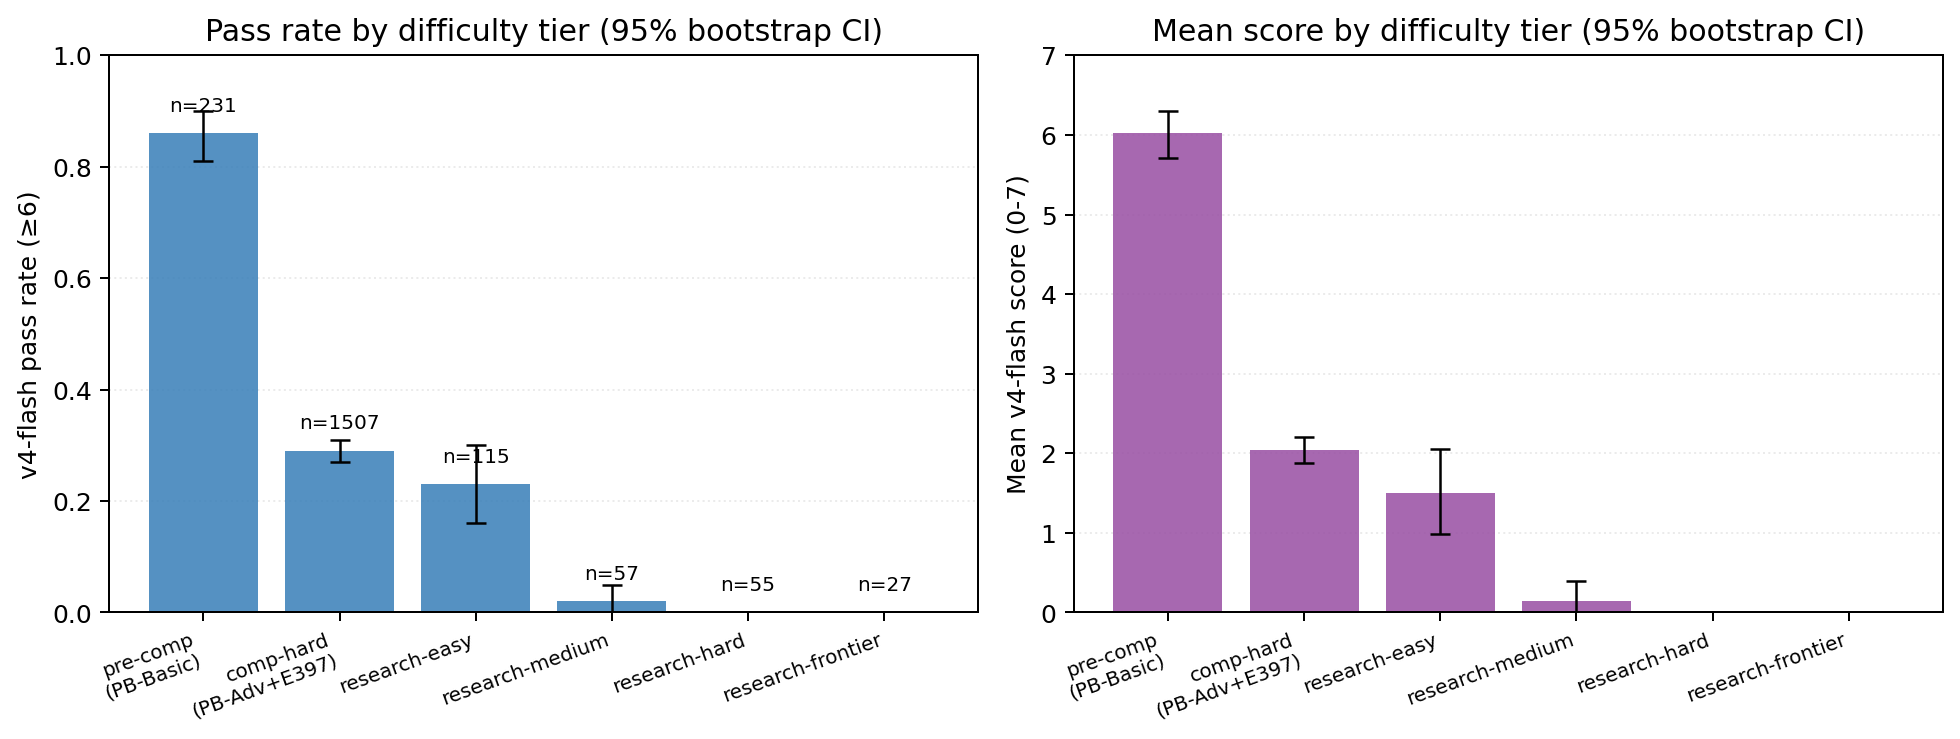
\includegraphics[width=0.85\textwidth]{plots/fig5_difficulty_gradient.png}
  \caption{Pass rate (left) and mean score (right) by difficulty tier with 95\%
    bootstrap CIs. Strict-judge pass rate falls from 86\% at PB-Basic to 0\% at
    research-hard and above.}
  \label{fig:difficulty}
\end{figure}

Architecture lift is null on hard tiers under strict judges.
\texttt{full}~$-$~\texttt{generate} is null at every tier (R26-only
$\Delta{=}{+}0.06$, $p{=}1.0$).
\texttt{seed\_full}~$-$~\texttt{generate} on R26 is $+0.48$ [$-$0.03, $+$1.14]
($n{=}42$, cluster $p{=}0.38$), directionally positive but not significant.
Figure~\ref{fig:lift} shows the lift-by-tier forest plot.

\subsection{Judge choice flips the cheap-model comparison}
\label{sec:judges}

The same raw outputs scored by Gemini-3-flash-preview tell a different story
(Figure~\ref{fig:judge}).
Under Gemini, four of six models show $+0.14$ to $+0.83$ lift from the pipeline;
the strict judges show no such pattern.
On the 1{,}440 cells where all three judges scored:
strict judges agree on 95.5\% [94.4, 96.5] of pass/fail decisions.
$P(\text{Gemini pass} \mid \text{v4-flash fail}) = 0.37$ [0.34, 0.40]
over $n{=}987$ strict-fail cases---a systematic offset, not
noise~\citep{zheng2023llmjudge}.
The reverse, $P(\text{Gemini fail} \mid \text{v4-flash pass}) = 0.035$, over
$n{=}453$.
We use v4-flash for headline numbers.

\begin{figure}[t]
  \centering
  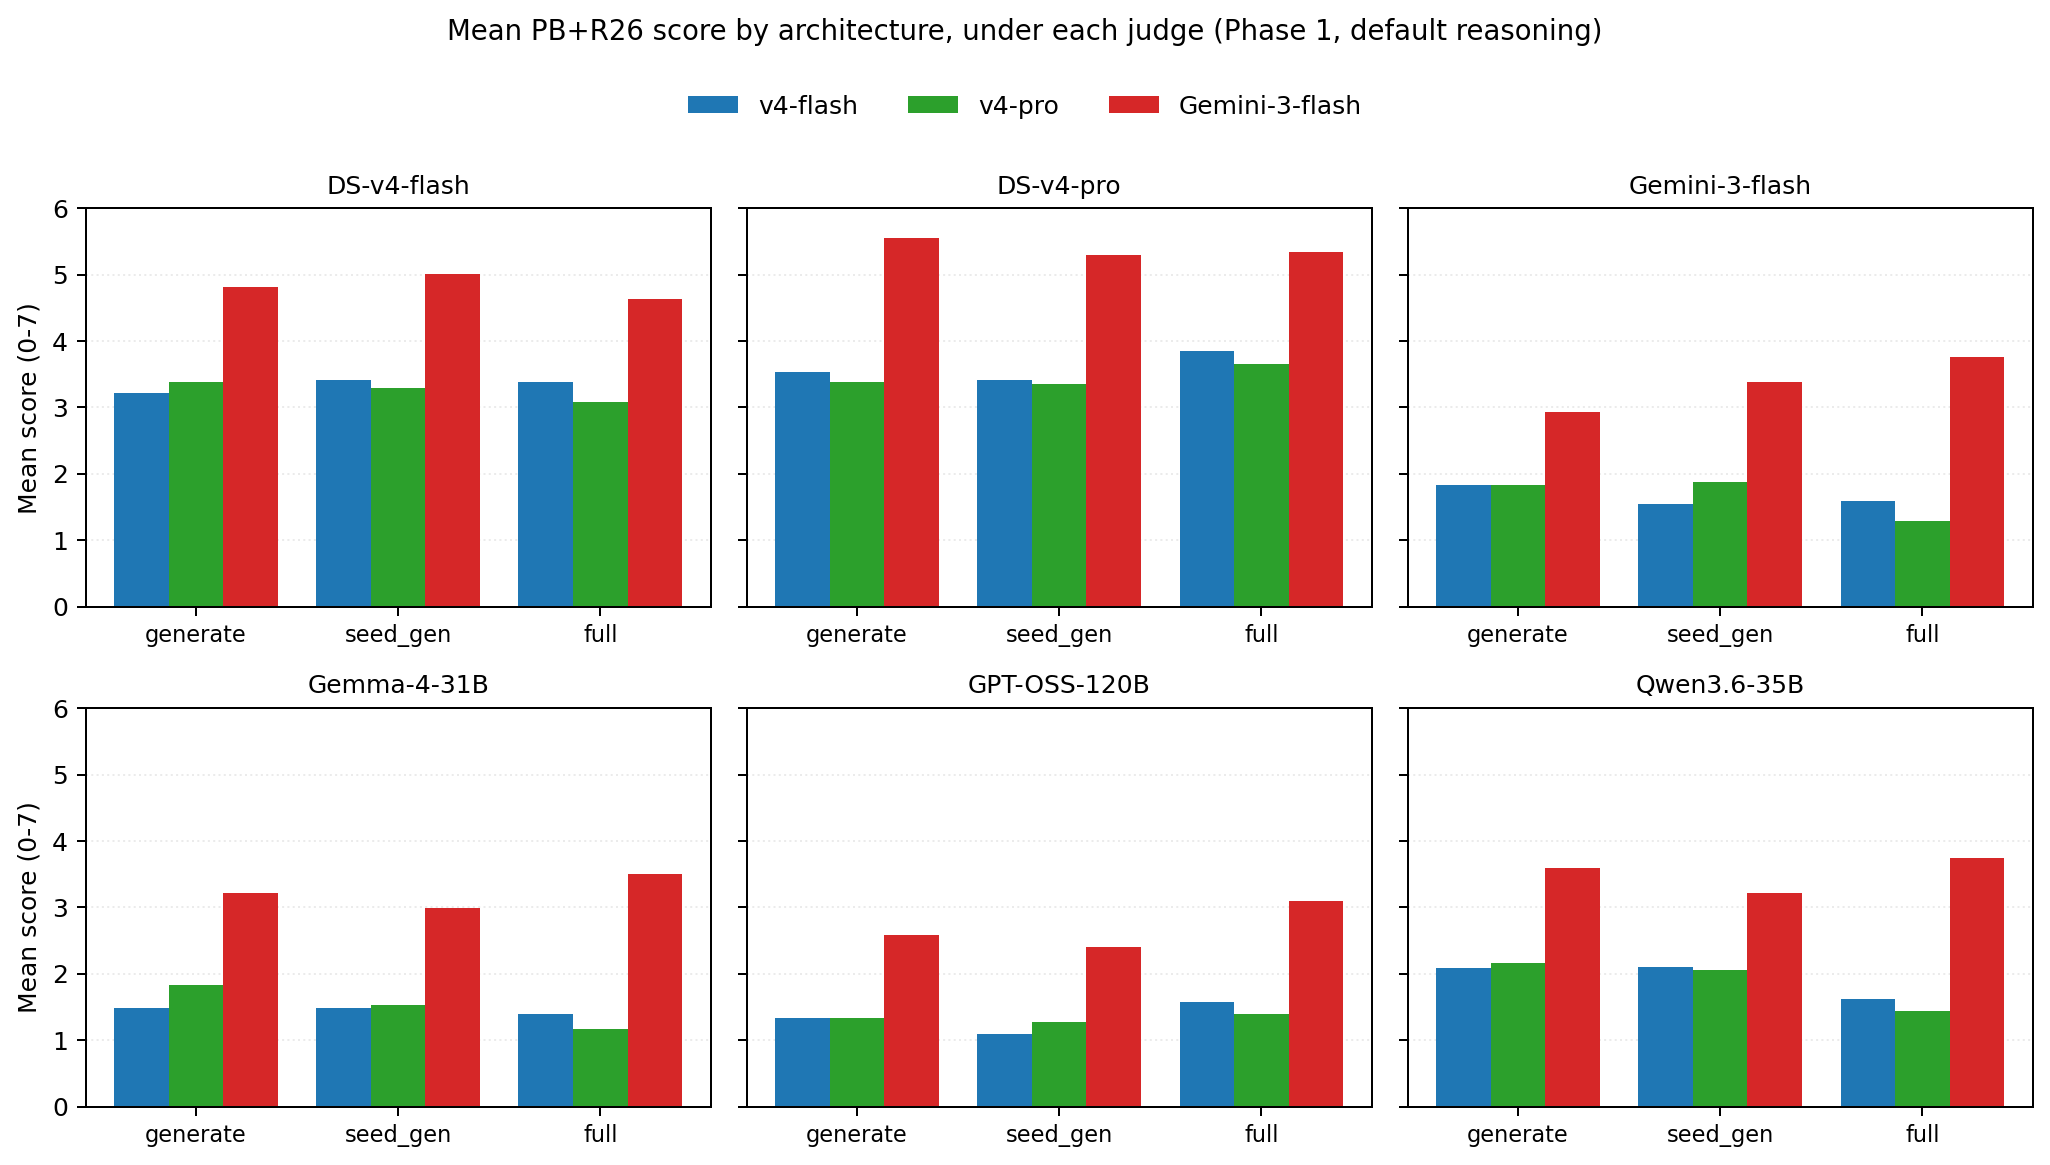
\includegraphics[width=0.95\textwidth]{plots/fig1_judge_sensitivity.png}
  \caption{Mean PB+R26 score by architecture under each of three judges, for each
    base model (Phase~1, default reasoning). The lenient judge (Gemini, red)
    systematically inflates pipeline scores on weaker models.}
  \label{fig:judge}
\end{figure}

\paragraph{Generator-judge family check.}
The v4-flash judge shares family with two generators (DeepSeek-v4-flash, -pro).
For \texttt{seed\_full}~$-$~\texttt{generate}, same-family $\Delta{=}{+}0.15$
[$-$0.49, $+$0.79]; different-family $\Delta{=}{+}0.35$ [$+$0.09, $+$0.62].
The lift is concentrated in cross-family generators, so judge-family bias does not
drive the headline (Appendix~\ref{app:family}).

\subsection{Where seeded-ideator-plus-pipeline helps}
\label{sec:seedfull}

The pooled \texttt{seed\_full}~$-$~\texttt{generate} lift (+0.32, $p{=}0.006$) is
over a non-representative model subset and heavily confounded by reasoning.
Stratifying (Table~\ref{tab:seedfull}):

\begin{table}[t]
  \caption{\texttt{seed\_full}~$-$~\texttt{generate} lift stratified by reasoning
    mode (problem-clustered CIs).}
  \label{tab:seedfull}
  \centering
  \small
  \begin{tabular}{lrrrl}
    \toprule
    Stratum & $n$/problems & $\Delta$ & cluster 95\% CI & $p$ \\
    \midrule
    default reasoning & 203\,/\,70 & +0.13 & [$-$0.14,\,+0.42] & 0.39 \\
    reasoning=max & 134\,/\,70 & \textbf{+0.60} & \textbf{[+0.21,\,+1.03]} & \textbf{0.005} \\
    \bottomrule
  \end{tabular}
\end{table}

The lift is entirely driven by reasoning=max cells.
Eight per-cell paired tests (Appendix~\ref{app:percell}) yield no cell surviving
Holm correction at $\alpha{=}0.05$ (smallest Holm-$p$~$=$~$0.15$); the
pooled-stratum cluster contrast survives ($p{=}0.005$).

\paragraph{Cost-matched comparison.}
At measured 1.36$\times$ generate cost, \texttt{seed\_full} is closer to pass@4--5.
Pass@5 means under v4-flash are 3.05 (Gemma max) and 2.83 (GPT-OSS max) vs.\
\texttt{seed\_full} 3.31 and 3.00: a small edge for cheap models at reasoning=max.
DeepSeek-v4-flash's pass@5 of 4.18 cleanly beats its \texttt{seed\_full} of 3.49.
Pure scaling wins for stronger generators.

\subsection{Frontier candidate passes}
\label{sec:frontier}

We use ``candidate pass'' throughout: every count is an automated-judge pass
not validated by an expert.
Pooling all 3{,}178 v4-flash-judged trials across architecture (2{,}098) and
scaling (1{,}080) experiments, Table~\ref{tab:frontier} shows per-problem results.

\begin{table}[t]
  \caption{R26 candidate passes per problem, pooling all experiments. Each problem
    has $\sim$33 cells. $\dagger$FirstProof-10 likely inflated by leaked solution direction.}
  \label{tab:frontier}
  \centering
  \small
  \begin{tabular}{llrrrrrr}
    \toprule
    Problem & Difficulty & cells & \multicolumn{2}{c}{v4-flash} & \multicolumn{2}{c}{Gemini} \\
    \cmidrule(lr){4-5} \cmidrule(lr){6-7}
    & & & pass & rate & pass & rate \\
    \midrule
    FirstProof~10$\dagger$ & res.-easy & 33 & 23 & 70\% & 8 & 24\% \\
    Erd\H{o}s~654 & res.-easy & 33 & 5 & 15\% & 6 & 18\% \\
    Erd\H{o}s~333 & res.-easy & 33 & 1 & 3\% & 2 & 6\% \\
    Erd\H{o}s~659 & res.-easy & 33 & 1 & 3\% & 7 & 21\% \\
    Erd\H{o}s~397 & comp.-hard & 33 & 1 & 3\% & 1 & 3\% \\
    FirstProof~5 & res.-med. & 33 & 1 & 3\% & 1 & 3\% \\
    Erd\H{o}s~1051 & res.-med. & 33 & 1 & 3\% & 14 & 42\% \\
    FirstProof~6 & res.-hard & 33 & 1 & 3\% & 5 & 15\% \\
    FirstProof~4 & res.-hard & 32 & 0 & 0\% & 1 & 3\% \\
    Ramsey & res.-front. & 33 & 0 & 0\% & 3 & 9\% \\
    \bottomrule
  \end{tabular}
\end{table}

Excluding FirstProof-10: 9~v4-flash candidate passes, 5 on Erd\H{o}s-654
(spanning four base models), plus single cells on six other problems including the
only strict candidate passes of Erd\H{o}s-1051 and FirstProof-6 (both
DeepSeek-v4-flash pass@7).
For Erd\H{o}s-1051, Gemini awards 14 passes against the strict judges' single
(v4-flash) and zero (v4-pro)---a sharp illustration of judge fragility.
The defensible reading of any single strict-judge candidate pass at
research-medium-or-harder difficulty is ``candidate for expert review,'' not
``confirmed solve.''

\begin{figure}[t]
  \centering
  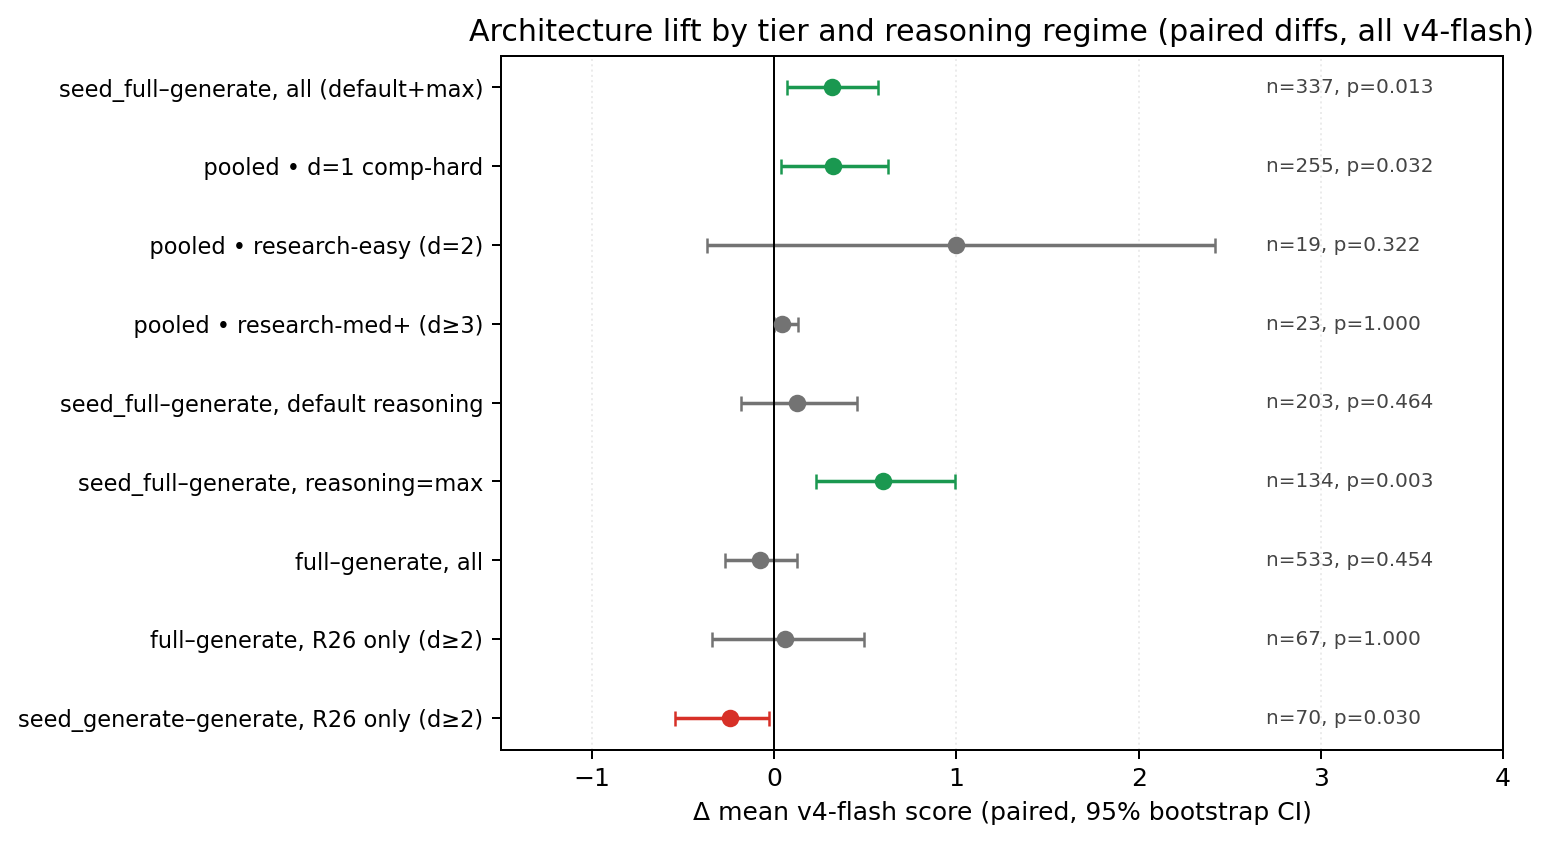
\includegraphics[width=0.9\textwidth]{plots/fig6_lift_by_tier.png}
  \caption{Architecture lift (paired $\Delta$ in v4-flash mean score) stratified by
    tier and reasoning regime. Green: significant at $p < 0.05$; grey: null; red:
    significant negative.}
  \label{fig:lift}
\end{figure}

%% ============================================================
\section{Secondary results}
\label{sec:secondary}

\paragraph{Reasoning effects exceed architecture effects.}
Reasoning-on adds $+0.78$ to $+1.60$ to v4-flash mean score (Gemma and GPT-OSS;
Appendix~\ref{app:reasoning}), 3--5$\times$ larger than architecture deltas.
This is well-established~\citep{wei2022cot,openai2024o1}; we present it as
confirmation, not discovery.

\paragraph{Pass@$k$ scales significantly through $k{=}9$.}
The scaling experiment computes pass@$n$ by exhaustive enumeration over all
size-$n$ subsets of the $M$ available samples (Figure~\ref{fig:passk}); a recent
extension to $M{=}9$ across all five cells gives pass@9 numbers directly, not
by extrapolation. Pass@9 means: DS-v4-flash default 4.54, Gemma-max 3.29,
GPT-OSS-max 3.23, Gemma-default 2.41, GPT-OSS-default 1.71. All pass@9$-$pass@3
deltas are positive and significant (paired bootstrap, $p{<}0.001$ in every cell);
pass@9$-$pass@7 deltas remain positive ($+0.08$ to $+0.22$, all $p{\le}0.0004$),
so the slope has not flattened by $k{=}9$.
Under the (generous) assumption that \texttt{seed\_full}'s nominal $\sim$9 calls
match pass@9 token-for-token, pure pass@9 ties Gemma-max \texttt{seed\_full}
(3.29 vs 3.31) and beats every other cell --- DS-flash default by $+1.05$,
GPT-OSS-max by $+0.23$, Gemma-default by $+0.70$, GPT-OSS-default by $+0.30$.
With the empirical cost matching above (\texttt{seed\_full} $\approx$ pass@4--5),
the gap is wider still.

\begin{figure}[t]
  \centering
  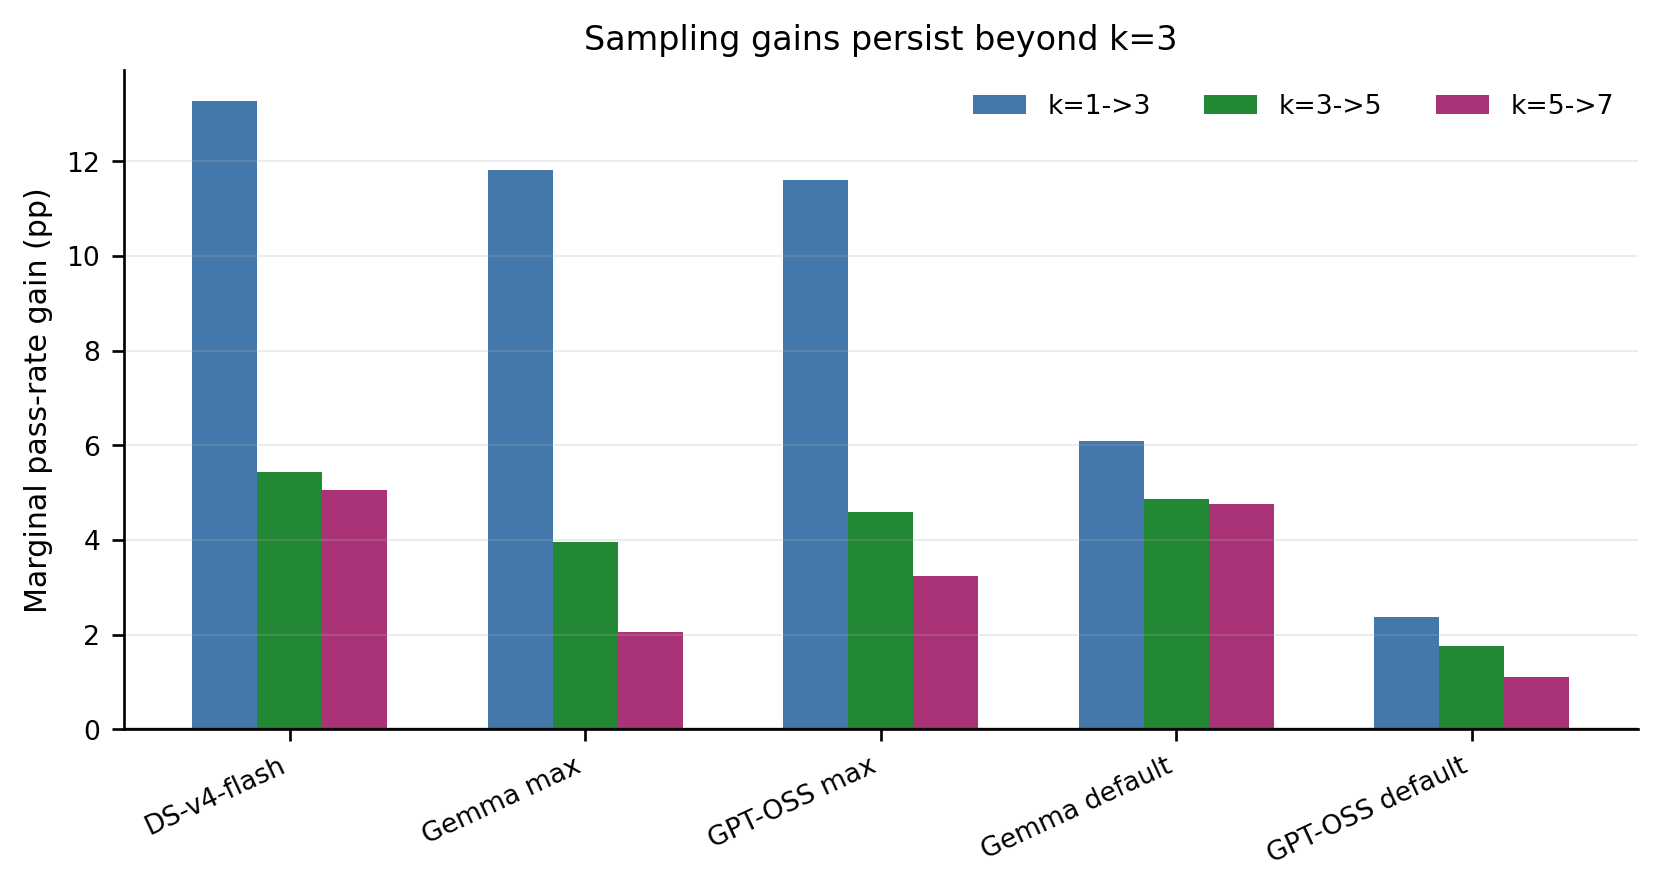
\includegraphics[width=0.7\textwidth]{plots/fig3_marginal_passn_gains.png}
  \caption{Marginal pass-rate gains from additional samples. The $k{=}1{\to}3$ step
    dominates, but $k{=}3{\to}5$ and $k{=}5{\to}7$ persist, especially for
    DS-v4-flash and cheap models at default reasoning.}
  \label{fig:passk}
\end{figure}

\paragraph{Cross-model role-swap is null.}
Varying which model fills each pipeline role in \texttt{seed\_full} at reasoning=max
yields eight conditions spanning 2.96--3.63 mean; only GPT-OSS-as-verifier (3.63)
beats both random baselines (3.19, 3.34).
The ``diversity helps'' hypothesis is not supported (Appendix~\ref{app:roleswap}).

\paragraph{Coverage asymmetry.}
Three base models (DeepSeek-v4-pro, Gemini-3-flash-preview, Qwen3.6) lack
\texttt{seed\_full} runs due to budget constraints.
Closing this gap is the single largest follow-up the budget left on the table.

%% ============================================================
\section{Limitations}
\label{sec:limitations}

\paragraph{Benchmark contamination.}
Most R26 solution-disclosure dates fall in 2026.
Several generators have post-training cutoffs that overlap (Gemma-4: March~31;
DeepSeek-v4: April~24).
GPT-OSS-120B (released August~2025) is provably contamination-free for every R26
solution.
Solve patterns for GPT-OSS and DeepSeek look broadly similar, which we read as
weak evidence that contamination is not the dominant signal.

\paragraph{Judging.}
Calibrated to $\sim$87\% pass-agreement on GradingBench (IMO-class items); judge
accuracy on Erd\H{o}s/First-Proof material is an extrapolation.
Section~\ref{sec:frontier}'s candidate-pass counts of 1/33 are candidates for
expert review, not confirmed mathematics.

\paragraph{Generalization.}
Our models top out at DeepSeek-v4-pro.
We do not test frontier-tier models on the full sweep, though a small probe
(Appendix~\ref{app:expensive}) suggests Kimi-k2.6 deserves a future look.

\paragraph{Dataset size.}
$n{=}70$ is small; only ten problems are research-grade, with $n{=}2$--4 per tier
at research-medium-and-harder.

\paragraph{Single-judge audit.}
The cleanest pipeline-lift result (\S\ref{sec:seedfull}) is v4-flash only; a v4-pro
audit would strengthen the claim.

\paragraph{Multiple comparisons.}
Per-cell tests do not survive Holm at $\alpha{=}0.05$; the pooled reasoning=max
stratum contrast ($p{=}0.005$) is the load-bearing positive.

\paragraph{AI-assistance.}
Drafts were prepared with LLM assistance for prose and analysis-script
scaffolding.
All numerical results were computed by the referenced analysis scripts.

%% ============================================================
\section{Discussion}
\label{sec:discussion}

Three takeaways.

\paragraph{The verifier-revisor pipeline does not beat call-matched sampling.}
Across 533 paired cells, \texttt{full}~$-$~\texttt{generate} is null
($\Delta{=}{-}0.08$, $p{=}0.36$).
Seeded-ideator-plus-pipeline shows a positive effect concentrated in reasoning=max
cheap-model cells ($\Delta{=}{+}0.60$, $p{=}0.005$); at default reasoning the
effect is null; per-cell tests do not survive Holm correction.
The recommendation: draw more samples before adding pipeline depth, keep reasoning
on, use a calibrated judge.

\paragraph{Audit with judges of different leniency.}
Strict judges agree on 95.5\% of decisions; Gemini calls ``pass'' on 37\% of
strict-fail cases.
A two-judge audit is a cheap discipline.

\paragraph{Frontier candidate passes are concentrated and judge-fragile.}
Pooling 3{,}178 trials yields 32 strict-judge R26 candidate passes; 23 on
FirstProof-10 (likely contaminated).
Excluding it: 9 candidate passes, 5 on Erd\H{o}s-654.
A candidate pass from a cheap model on a research-medium-or-harder problem is a
flag for expert review, not a theorem.

\paragraph{Budget and follow-ups.}
Results came from {\raise.17ex\hbox{$\scriptstyle\sim$}}\$800 of inference.
{\raise.17ex\hbox{$\scriptstyle\sim$}}\$20 of v4-pro grades on the four reasoning=max
\texttt{seed\_full} cells would harden \S\ref{sec:seedfull}'s result.
A Phase-1 \texttt{seed\_full} extension on three missing base models closes the
largest coverage gap.
A fair pass@$k$-vs-pipeline comparison at frontier models would test whether the
cheap-model finding generalizes.

\paragraph{Resources and audit.}
Architecture sweep: 2{,}098 trials $\times$ 6 base models.
Scaling: 1{,}080 trials.
Aggregate API spend {\raise.17ex\hbox{$\scriptstyle\sim$}}\$800 against a \$1{,}000 budget.
Known data-quality issue: original Phase~1 seeded-ideator runs had
$\sim$10--28\% malformed-ideator outputs that silently fell back to pass@3,
which would \emph{understate} any seeded-ideator effect; we patched the bug for
Phase~2 onward.


%% ============================================================

\begin{ack}
This work was supported by a personal research budget of \$1{,}000 for API
inference costs via OpenRouter. No external funding was received.
\end{ack}

%% ============================================================

{\small
\bibliographystyle{plainnat}
\bibliography{references}
}

%% ============================================================
\appendix

\section{GradingBench full table}
\label{app:gradingbench}

Ten judge configurations on $n{=}200$ from GradingBench, sorted by pass-agreement at 6.

\begin{table}[h]
  \centering
  \small
  \begin{tabular}{llrrrrrrrl}
    \toprule
    Judge & Reasoning & $n$ & pass$\geq$6 & recall & spec & F1 & $r$ & \$/call & lat. \\
    \midrule
    GPT-5.4-nano & xhigh & 196 & 89.3\% & 70\% & 98\% & 0.800 & 0.711 & \$0.037 & 152s \\
    DS-v4-pro & default & 198 & 88.9\% & 83\% & 92\% & 0.825 & 0.756 & \$0.015 & 299s \\
    DS-v4-flash & default & 199 & 87.4\% & 79\% & 91\% & 0.800 & 0.756 & \$0.004 & 81s \\
    Gemini-3.1-pro & default & 199 & 86.4\% & 95\% & 82\% & 0.816 & 0.872 & \$0.035 & 22s \\
    GPT-OSS-120B & xhigh & 178 & 84.3\% & 90\% & 82\% & 0.788 & 0.770 & \$0.002 & 62s \\
    DS-v4-flash & reas.\ off & 192 & 80.7\% & 56\% & 92\% & 0.654 & 0.591 & \$0.002 & 13s \\
    Gemma-4-31B & high & 200 & 79.0\% & 92\% & 73\% & 0.734 & 0.776 & \$0.004 & 126s \\
    GPT-OSS-120B & default & 199 & 71.9\% & 74\% & 71\% & 0.622 & 0.513 & \$0.001 & 9s \\
    Gemma-4-31B & default & 200 & 65.5\% & 98\% & 50\% & 0.642 & 0.629 & \$0.002 & 19s \\
    Gemini-3-flash & default & 200 & 64.0\% & 98\% & 48\% & 0.633 & 0.606 & \$0.016 & 4s \\
    \bottomrule
  \end{tabular}
\end{table}

\section{AnswerBench-50 generator calibration}
\label{app:answerbench}

\begin{table}[h]
  \centering
  \small
  \begin{tabular}{llrl}
    \toprule
    Model & Config & Accuracy & Notes \\
    \midrule
    DeepSeek-v4-pro & default & 94\% (47/50) & top accuracy \\
    GPT-5.4-nano & xhigh & 92\% (45/49) & 1 hung \\
    Gemini-3-flash & xhigh (synth) & 90\% (45/50) & \\
    DeepSeek-v4-flash & default & 88\% (44/50) & best value \\
    Qwen3.6-35B-A3B & default & 80\% (40/50) & \\
    GPT-OSS-120B & xhigh & 74\% (37/50) & +16pp vs default \\
    Gemini-3-flash & default & 74\% (37/50) & \\
    Gemma-4-31B-IT & default & 68\% (34/50) & reas.\ off \\
    GPT-OSS-120B & default & 58\% (29/50) & \\
    DS-v4-flash & reasoning off & 50\% (25/50) & $-$38pp \\
    \bottomrule
  \end{tabular}
\end{table}

\section{Per-cell means (architecture $\times$ judge $\times$ model)}
\label{app:percell_means}

\begin{table}[h]
  \centering
  \small
  \begin{tabular}{llrrr}
    \toprule
    Model $\times$ Mode & Reas. & v4-flash & v4-pro & Gemini \\
    \midrule
    DS-v4-flash $\times$ generate & def & 3.22 & 3.39 & 4.81 \\
    DS-v4-flash $\times$ seed\_gen & def & 3.41 & 3.30 & 5.01 \\
    DS-v4-flash $\times$ full & def & 3.38 & 3.09 & 4.63 \\
    DS-v4-flash $\times$ seed\_full & def & 3.49 & 3.19 & 5.83 \\
    DS-v4-pro $\times$ generate & def & 3.53 & 3.38 & 5.56 \\
    DS-v4-pro $\times$ seed\_gen & def & 3.41 & 3.36 & 5.30 \\
    DS-v4-pro $\times$ full & def & 3.85 & 3.66 & 5.35 \\
    Gemini-3-flash $\times$ generate & def & 1.83 & 1.83 & 2.93 \\
    Gemini-3-flash $\times$ seed\_gen & def & 1.54 & 1.87 & 3.39 \\
    Gemini-3-flash $\times$ full & def & 1.59 & 1.29 & 3.76 \\
    Gemma-4 $\times$ generate & def & 1.49 & 1.83 & 3.21 \\
    Gemma-4 $\times$ seed\_gen & def & 1.49 & 1.53 & 2.99 \\
    Gemma-4 $\times$ full & def & 1.39 & 1.17 & 3.51 \\
    Gemma-4 $\times$ seed\_full & def & 1.71 & 1.67 & 4.26 \\
    Gemma-4 $\times$ generate & max & 2.74 & -- & -- \\
    Gemma-4 $\times$ seed\_full & max & 3.31 & -- & -- \\
    Gemma-4 $\times$ full & max & 2.17 & -- & -- \\
    GPT-OSS $\times$ generate & def & 1.34 & 1.33 & 2.59 \\
    GPT-OSS $\times$ seed\_gen & def & 1.09 & 1.27 & 2.40 \\
    GPT-OSS $\times$ full & def & 1.58 & 1.39 & 3.10 \\
    GPT-OSS $\times$ seed\_full & def & 1.41 & 1.37 & 3.99 \\
    GPT-OSS $\times$ generate & max & 2.30 & -- & -- \\
    GPT-OSS $\times$ seed\_full & max & 3.00 & -- & -- \\
    GPT-OSS $\times$ full & max & 2.43 & -- & -- \\
    Qwen3.6 $\times$ generate & def & 2.09 & 2.17 & 3.60 \\
    Qwen3.6 $\times$ seed\_gen & def & 2.10 & 2.06 & 3.21 \\
    Qwen3.6 $\times$ full & def & 1.62 & 1.44 & 3.74 \\
    \bottomrule
  \end{tabular}
\end{table}

\section{Reasoning effect on PB+R26}
\label{app:reasoning}

\begin{table}[h]
  \centering
  \small
  \begin{tabular}{llrrrr}
    \toprule
    Model & Mode & default & max & $\Delta$ & 95\% CI \\
    \midrule
    Gemma-4 & generate & 1.49 & 2.74 & +1.25 & [+0.74, +1.77] \\
    Gemma-4 & seed\_full & 1.71 & 3.31 & +1.60 & [+1.07, +2.14] \\
    GPT-OSS & generate & 1.34 & 2.30 & +0.96 & [+0.46, +1.46] \\
    GPT-OSS & seed\_full & 1.41 & 3.00 & +1.59 & [+1.05, +2.13] \\
    \bottomrule
  \end{tabular}
\end{table}

\section{Expensive-models probe}
\label{app:expensive}

$n{=}12$ problems, default reasoning.

\begin{table}[h]
  \centering
  \small
  \begin{tabular}{lrrl}
    \toprule
    Model & Accuracy & \$/run & Notes \\
    \midrule
    Kimi-k2.6 & 100\% (10/10) & \$0.097 & 2/12 hung \\
    Qwen3.6-Max & 92\% (11/12) & \$0.172 & dominated \\
    Gemini-3.1-Pro & 83\% (10/12) & \$0.250 & dominated \\
    GPT-5.4 & 50\% (6/12) & \$0.054 & artifact at default \\
    \bottomrule
  \end{tabular}
\end{table}

\section{Roleswap detail}
\label{app:roleswap}

\begin{table}[h]
  \centering
  \small
  \begin{tabular}{lrrr}
    \toprule
    Condition & $n$ & mean & pass rate \\
    \midrule
    random\_run1 & 69 & 3.19 & 0.45 \\
    random\_run2 & 70 & 3.34 & 0.49 \\
    x\_ideate\_gemma & 68 & 3.09 & 0.44 \\
    x\_ideate\_oss & 70 & 2.96 & 0.41 \\
    x\_revise\_gemma & 69 & 3.48 & 0.49 \\
    x\_revise\_oss & 70 & 3.41 & 0.49 \\
    x\_verify\_gemma & 69 & 3.00 & 0.43 \\
    \textbf{x\_verify\_oss} & 70 & \textbf{3.63} & \textbf{0.51} \\
    \bottomrule
  \end{tabular}
\end{table}

\section{Judge agreement rates}
\label{app:judgeagree}

\begin{table}[h]
  \centering
  \small
  \begin{tabular}{lrr}
    \toprule
    Pair & Agreement & 95\% CI \\
    \midrule
    v4-flash vs v4-pro & 95.5\% & [94.4, 96.5] \\
    v4-flash vs Gemini & 73.7\% & [71.5, 76.0] \\
    v4-pro vs Gemini & 72.9\% & [70.6, 75.3] \\
    \bottomrule
  \end{tabular}
\end{table}

\begin{table}[h]
  \centering
  \small
  \begin{tabular}{lrrr}
    \toprule
    Conditional flip & Estimate & 95\% CI & $n$ \\
    \midrule
    $P(\text{Gemini pass} \mid \text{v4-flash fail})$ & 0.368 & [0.338, 0.398] & 987 \\
    $P(\text{Gemini fail} \mid \text{v4-flash pass})$ & 0.035 & [0.020, 0.053] & 453 \\
    \bottomrule
  \end{tabular}
\end{table}

\section{Per-cell Holm-corrected tests}
\label{app:percell}

\begin{table}[h]
  \centering
  \small
  \begin{tabular}{lrrrr}
    \toprule
    Cell & $n$ & $\Delta$ & $p_{\text{raw}}$ & $p_{\text{Holm}}$ \\
    \midrule
    Gemma max, seed\_full $-$ gen & 70 & +0.57 & 0.039 & 0.275 \\
    GPT-OSS max, seed\_full $-$ gen & 64 & +0.63 & 0.046 & 0.278 \\
    Gemma max, full $-$ gen & 70 & $-$0.57 & 0.019 & 0.152 \\
    GPT-OSS max, full $-$ gen & 65 & +0.17 & 0.70 & 1.00 \\
    DS-v4-flash def, seed\_full $-$ gen & 66 & +0.15 & 0.71 & 1.00 \\
    DS-v4-pro def, full $-$ gen & 60 & +0.23 & 0.57 & 1.00 \\
    Gemma def, seed\_full $-$ gen & 69 & +0.14 & 0.56 & 1.00 \\
    GPT-OSS def, seed\_full $-$ gen & 68 & +0.09 & 0.86 & 1.00 \\
    \bottomrule
  \end{tabular}
\end{table}

\section{Empirical cost per architecture}
\label{app:cost}

\begin{table}[h]
  \centering
  \small
  \begin{tabular}{lrrrrr}
    \toprule
    Mode & $n$ & mean \$ & median \$ & p90 \$ & ratio \\
    \midrule
    generate (= pass@3) & 558 & 0.084 & 0.040 & 0.224 & 1.00$\times$ \\
    seed\_generate & 560 & 0.084 & 0.041 & 0.226 & 1.00$\times$ \\
    full & 560 & 0.066 & 0.030 & 0.129 & 0.78$\times$ \\
    seed\_full & 349 & 0.114 & 0.071 & 0.215 & 1.36$\times$ \\
    \bottomrule
  \end{tabular}
\end{table}

\section{Generator-judge family stratification}
\label{app:family}

Same family = DeepSeek generators; different family = all others.
v4-flash judge throughout.

\begin{table}[h]
  \centering
  \small
  \begin{tabular}{lrr}
    \toprule
    Contrast & Same family $\Delta$ [CI] & Different family $\Delta$ [CI] \\
    \midrule
    full $-$ gen & +0.11 [$-$0.29, +0.54] & $-$0.14 [$-$0.36, +0.09] \\
    seed\_gen $-$ gen & $-$0.05 [$-$0.47, +0.38] & $-$0.02 [$-$0.22, +0.17] \\
    seed\_full $-$ gen & +0.15 [$-$0.49, +0.79] & +0.35 [+0.09, +0.62] \\
    \bottomrule
  \end{tabular}
\end{table}

%% ============================================================
\newpage
\input{checklist}

\end{document}
